\chapter{BIPEDAL WALKING BY TWIN DELAYED DEEP DETERMINISTIC POLICY GRADIENTS}
\label{chap:exp_setup}

\section{Details of the Environment}

\textit{BipedalWalker-v3} and \textit{BipedalWalker-Hardcore-v3} are two simulation environments of a bipedal robot, 
with relatively flat course and obstacle course respectively. 
Dynamics of the robot are exactly identical in both environments. 
Our task is to solve hardcore version where the agent is expected to learn to run and walk in different road conditions. 
Components of the hardcore environment is visualized in \figref{fig:bipedal_hardcore_components}. 

\begin{figure}
	\centering
	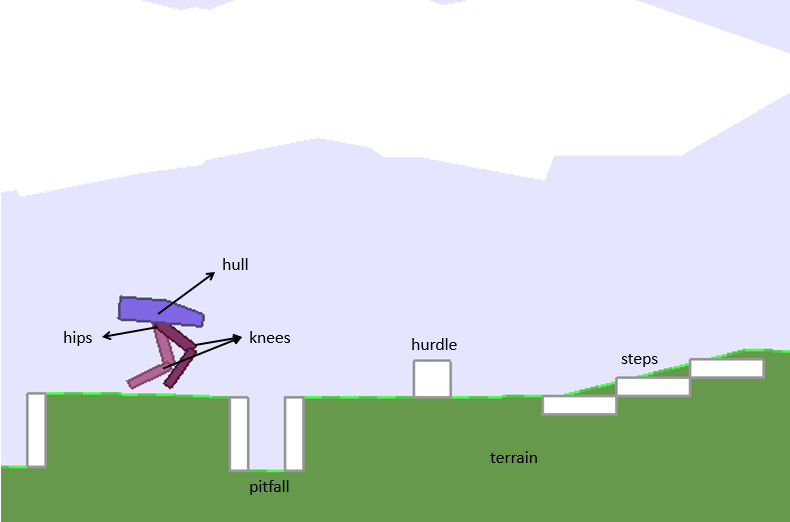
\includegraphics[width=0.95\textwidth]{figures/bipedal/bpedal_annotated.png}
	\caption{Bipedal Walker Hardcore Components~\cite{noauthor_bipedalwalkerhardcore-v2_2021}}
	\label{fig:bipedal_hardcore_components}
\end{figure}

The robot has kinematic and lidar sensors, and has deterministic dynamics.

\textbf{Observation Space} contains hull angle, hull angular velocity, hull translational velocities, joint positions, joint angular speeds, leg ground concats and ten lidar rangefinder measurements. Details and their constraints are summarized in \tabref{table:bpw_obs_space}. 

\begin{table}%[h!]
	\begin{center}
	\begin{tabular}{cccc}
		\textbf{Num} & \textbf{Observation} & \textbf{Interval} \\
		\hline 
		0  & Hull Angle & $[-\pi,\pi]$ \\
		1  & Hull Angular Speed & $[-\infty,\infty]$ \\
		2  & Hull Horizontal Speed & $[-1,1]$ \\
		3  & Hull Vertical Speed &$[-1,1]$ \\
		4  & Hip 1 Joint Angle & $[-\pi,\pi]$ \\
		5  & Hip 1 Joint Speed & $[-\infty,\infty]$ \\
		6  & Knee 1 Joint Angle & $[-\pi,\pi]$ \\
		7  & Knee 1 Joint Speed & $[-\infty,\infty]$ \\
		8  & Leg 1 Ground Contact Flag & $\{0,1\}$ \\
		9  & Hip 2 Joint Angle & $[-\pi,\pi]$ \\
		10  & Hip 2 Joint Speed & $[-\infty,\infty]$ \\
		11  & Knee 2 Joint Angle & $[-\pi,\pi]$ \\
		12  & Knee 2 Joint Speed & $[-\infty,\infty]$ \\
		13  & Leg 2 Ground Contact Flag & $\{0,1\}$ \\
		14-23  & Lidar measures  & $[-\infty,\infty]$
	\end{tabular}
	\end{center}
	\caption{Observation Space of Bipedal Walker}
	\label{table:bpw_obs_space}
\end{table}

The robot has two legs with two joints at knee and hip. Torque is provided to knee and pelvis joints of both legs. These four torque values forms the \textbf{Action Space}, presented in \tabref{table:bpw_act_space} with their constraints. 

\begin{table}%[h!]
	\begin{center}
		\begin{tabular}{cccc}
			\textbf{Num} & \textbf{Observation} & \textbf{Interval} \\
			\hline
			0  & Hip 1 Torque & $[-1,1]$ \\
			1  & Hip 2 Torque & $[-1,1]$ \\
			2  & Knee 1 Torque & $[-1,1]$ \\
			3  & Knee 2 Torque & $[-1,1]$ \\
		\end{tabular}
	\end{center}
	\caption{Action Space of Bipedal Walker}
	\label{table:bpw_act_space}
\end{table}

\textbf{Reward Function} is a bit complex in the sense that the robot should run fast with little energy while it should not stumble and fall to ground. 
Directly proportional to distance traveled forward, +300 points given if agent reaches to end of the path. 
However, -10 points (-100 points in the original version) if agent falls, 
and small amount of negative reward proportional to the applied motor torque (to prevent applying unnecessary torque). 
Lastly, the robots gets negative reward propotional to the absolute value of the hull angle for reinforcing to keep the hull straigth. 

\subsection{Partial Observability}

The environment is partially observable due to following reasons.
\begin{itemize}
	\item The agent is not able to track behind with the lidar sensor. 
	Unless it has a memory, it cannot know whether a pitfall or hurdle behind. 
	Illustration is shown in \figref{fig:partial_obs_pitfall}.
	\item There is no accelerometer sensor. 
	Therefore, the agent do not know whether it is accelerating or decelerating.
\end{itemize}

\begin{figure}
	\begin{subfigure}{.32\textwidth}
		\centering
		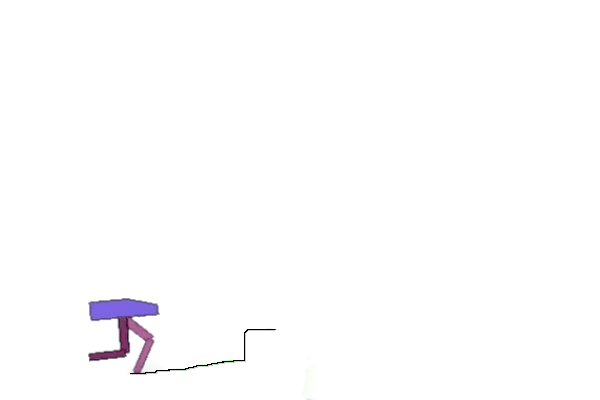
\includegraphics[width=0.99\linewidth]{figures/bipedal/po/lidarcover.png}
		\caption{Perspective}
		\label{fig:lidar_cover}
	\end{subfigure}
	\begin{subfigure}{.32\textwidth}
		\centering
		
\includegraphics[width=0.99\linewidth]{figures/bipedal/po/pitfall_behind.png}
		\caption{Pitfall Behind}
		\label{fig:pitfall_behind}
	\end{subfigure}
		\begin{subfigure}{.32\textwidth}
		\centering
		
\includegraphics[width=0.99\linewidth]{figures/bipedal/po/no_pitfall_behind.png}
		\caption{No Pitfall Behind}
		\label{fig:no_pitfall_behind}
	\end{subfigure}
	\caption{Perspective of agent and possible realities}
	\label{fig:partial_obs_pitfall}
\end{figure}

In DRL, partial observability is handled by two ways in literature~ \cite{dulac-arnold_challenges_2019}. 
The first is incorporating fixed number of last observations while the second way is updating hidden belief state using recurrent-like neural network at each time step. 
Our approach is somewhere in between. We pass fixed number of past observations into LSTM and Transformer networks for both actor and critic. 

\subsection{Reward Sparsity}

Rewards given to the agent is sparse in some circumstances, in the following sense:
\begin{itemize}
	\item Overcoming big hurdles requires a very specific move. 
	The agent should explore many actions when faced with a big hurdle.
	\item Crossing pitfalls also require a specific move but not as complex as big hurdles.
\end{itemize}

\subsection{Modifications on Original Envrionment}

It is difficult to find an optimal policy directly with available setting. 
There are few studies in the literature demonstrating a solution for \textit{BipedalWalker-Hardcore-v3}. 
The following modifications are proposed.

\begin{itemize}
	\item In original version, agent gets -100 points when its hull hits the floor. 
	In order to make the robot more greedy, this is changed to -10 points. 
	Otherwise, agent cannot explore environment since it gets too much punishment when failed and learns to do nothing.
	\item Time resolution of simulation is halved (from 50 Hz to 25 Hz) by only observing last of each two consecutive frames using a custom wrapper function. 
	Since there is not a high frequency dynamics, this allows nothing but speeding up the learning process.
	\item In original implementation, an episode has a time limit. 
	Once this limit is reached, simulation stops with terminal state flag. 
	On the other hand, when agent fails before the time limit, the episode ends with terminal state flag too. 
	In the first case, the terminal state flag causes instability since next step's value is not used in value update, since it is not a logical terminal, just time up indicator.
	The environment changed such that terminal state flag is not given in this case unless agent fails. 
\end{itemize}

Once those modifications are applied on the environment, we observed quite improvement on both convergence and scores. 
